\section{Approach}
\label{sec:appro}
Our general approach is based on an SVM classifier using a hybrid
kernel function which combines a novel random walk graph kernel and a normal
radial basis function (RBF) \cite{Buhmann:RBF}. The graph kernel assesses
the similarity between different propagation trees while the RBF
kernel computes the distance between two vectors of both traditional and
high level semantic features. In this section, we will first introduce
the labeled propagation tree structure as well as
the random walk kernel, then present 8 new features used in the RBF
kernel, and finally show how to combined the two kernels into a hybrid
SVM kernel.
%
%In our study, each message, which need to be classified, is represented as a vector that every element corresponds to a feature.
%Some features are proposed by us while others are proposed by previous work.
%The combined kernel includes
%kernel and random walk graph kernel.
%The RBF kernel is used for vectors which is the traditional part of SVM.
%The random walk graph kernel is used to calculate the similarity of propagation tree, which is a new method proposed by us.

\subsection{Propagation tree}
\label{sec:tree}
For the purpose of the random walk graph kernel, we enrich the propagation tree
in \figref{fig:ptree} by adding additional information
which represents the type of user of each message and the opinion and
sentiment toward the original message. The resulting
propagation tree\footnote{Note that this data structure contains only part
of the information contained in the message propagation tree model in \secref{sec:prob}. The remaining information will be used in the RBF kernel.} will be used in the graph kernel computation.

We divide the users into two types: {\em opinion leaders} and
{\em normal users}. Opinion leaders are those influential users whose
opinions dominate their followers\cite{bodendorf2009detecting}.
A user is considered an opinion leader if
\begin{equation}
\frac{\rm{\#~ of~ followers}}{\rm{\#~ of~ friends}} > \alpha
\label{eq:alpha}
\end{equation}
where $\alpha > 1$ and \# of followers $\ge 1000$.
We thus label each node of the tree as $p$ if it comes from
an opinion leader and $n$ otherwise.

We label the edge from $m_i$ to $m_j$, called $e_{j}$\footnote{Since the
parent of $m_j$ is unique, $e_j$ uniquely identifies the edge
between $m_j$ and its parent.}, with a triple
$\boldsymbol{v_j} = (\theta(a),\theta(d),\theta(s))$,
where $a$ is the {\em approval score}
of $m_j$, which indicates approval or agreement,
$d$ is the {\em doubt score} of $m_j$ which indicate doubts and suspicion,
and $s$ is the overall sentiment score in $m_j$.
We defer the computation of $a$, $d$ and $s$ to \secref{sec:feature}.
$\theta$ is a damping function defined by
\begin{equation}
\theta(x) = 2^{-\rho t} x
\end{equation}
where $t$ is the time difference in days between the original message
and $m_j$, and $\rho$ is a parameter between 0 and 1.
The idea is: the sooner a user gives a response, the more intense
the response is.
%So the label of $e_i$ can reflect the sentiment and the intensity of
%user $u_i$'s option toward the original message $m_1$.
\figref{fig:ltree} shows such a labeled propagation tree in which
all reposts are sent in the same day as the original message. Once
the triple is extracted from the message, message id $m_i$ can be removed
from the nodes for simplicity.
%In the example illustrated before , if $u_1, u_2$ are opinion leaders, $u_3, u_4, u_5$ are normal users and all messages reposted in the first day then it can be represented as figure \ref{fig:4}.
\begin{figure}[htb]
\centering
\epsfig{file=ptree_ex2.eps, width=0.5\columnwidth}
\caption{Example of Labeled Propagation Tree}
\label{fig:ltree}
\end{figure}

Our intuition is that patterns can be discovered from
the labeled propagation tree,
which helps distinguish false rumors from others. For example,
\figref{fig:patterns} compares the partial labeled trees rooted from the two
messages about rove beetles in \figref{fig:beetle-rumor} and
\figref{fig:beetle-truth}. Despite the lexical similarity of the two
original messages, the false rumor (a) is reposted and supported by many
opinion leaders at first before normal users take over the propagation;
conversely the normal message (b) is initially reposted by a majority of
normal users. This shows that the influence of multiple opinion leaders can
quickly create a ``hype'' which is followed by ordinary users.

\begin{figure}[th]
\centering
\epsfig{file=ptree_ex4.eps, width=0.7\columnwidth}
\caption{Tree of False Rumors and Others}
\label{fig:patterns}
\end{figure}

In a social network with 50 million active users, a popular message can be
reposted thousands of times and the propagation tree thus gets extremely large.
To reduce the computation complexity of graph kernel function, we develop
the following rules to simplify a tree by lumping adjacent
normal user nodes together to form one {\em super node}, and thus
reduce \figref{fig:patterns}(b) to \figref{fig:simplified}:
\begin{enumerate}
\item If $m_i$ is the parent of $m_j$, and both are labeled as $n$,
then $m_i$, $m_j$ merge into one node $m_{ij}$,
whose parent is the parent of
$m_i$ and whose children are the children of $m_i$ or $m_j$;
\item If $m_i$ is sibling of $m_j$ and both are labeled as $n$ then
$m_i,m_j$ merge into one node $m_{ij}$, whose parent is the parent of
$m_i$ and $m_j$, and whose children are the children of $m_i$ or $m_j$;
\item The merged node $m_{ij}$ has label $n$ and the
label of incoming edge
$e_{ij}$ is $\boldsymbol{v_{ij}} = \boldsymbol{v_i} + \boldsymbol{v_j}$;
\item Do not merge the root with any other nodes;
\item Repeat the above rules until no pair of nodes can be merged;
\item For each super node, normalize the vector on incoming edge
by the number of ordinary nodes merged into this super node.
\end{enumerate}

\begin{figure}[th]
\centering
\epsfig{file=ptree_ex3.eps, width=0.4\columnwidth}
\caption{Simplified Propagation Tree}
\label{fig:simplified}
\end{figure}

\subsection{Random walk graph kernel}
\label{sec:random}
%Since one message $M_i$ and its repost message can be represented as a tree $T_i$, our problem turns to classify $\{T_i\}$ into two sets $R$ and $N$ where $R = \{T_i:T_i\textrm{ is a rumor}\}, S = \{T_i:T_i\textrm{ is a non-rumor}\}$. So we need to measure the similarity of two trees.

To classify different propagation trees by SVM, we need to calculate the
similarity between trees. There are several tree kernel functions that
can be used to calculate the similarity of trees such as the subset tree
(SST) kernel\cite{collins2002new} and subtree (ST) kernel\cite{smola2002fast}.
While these kernels prove to be useful in natural language
processing\cite{moschitti2006making}, they can not be used for our problem
because they consider two nodes to be similar only when they have the same
number of children. Whereas in this paper, if $m_i$ is reposted $a$ times
and $m_j$ is reposted $b$ times we would like to consider them similar
to some extent.

Instead of tree kernel, we use a random walk graph kernel
\cite{gartner2003graph} to calculate the similarity of trees. Because
the labels of edges in the propagation tree are not discrete values but
continuous vectors, we modify the original random walk kernel so that
the kernel is applicable to graphs with continuously labeled
edges\cite{neuhaus2006random}.

Given two trees $T=(V,E)$ and $T'=(V',E')$, we first calculate the direct product graph of two trees. The direct product graph of two trees is $G_\times = (T \times T') = (V_\times,E_\times)$, where
\begin{equation}
%\begin{displaymath}
\begin{aligned}
&V_\times = \{(v,v')\in V\times V':label(v)=label(v')\}\\
&E_\times = \{((u,u'),(v,v'))\in V_\times^2:\\
&\qquad\quad\ (u,v)\in E \wedge(u',v')\in E'\}
\end{aligned}
%\end{displaymath}
\end{equation}

The adjacency matrix of the direct product graph $G_\times$ is $A_\times$, which is defined as
$[A_\times]_{(u,u'),(v,v')} =l$, where
\begin{equation}
l =\left\{ \begin{array}{ll}
k((u,u'),(v,v'))& \mbox{if~} ((u,u'),(v,v'))\in E_\times,\\
0& \mbox{otherwise.}
\end{array}\right.
\end{equation}
The kernel function $k$ measures the similarity of edges $e_{(u,v)}$ and $e_{(u',v')}$,
and is given by
\begin{equation}
\begin{aligned}
k((u,u'),(v,v')) &= k_{edge}((u,v),(u',v'))\\
                 &= e^{-\frac{\|\boldsymbol{v_1}- \boldsymbol{v_2}\|^2}{2\sigma^2}}
\end{aligned}
\end{equation}
where $\boldsymbol{v_1}$ is the vector label of $e_{(u,v)}$, $\boldsymbol{v_2}$ is the vector label of $e_{(u',v')}$, and $\sigma$ is a parameter.\\

Given the adjacency matrix $A_\times$ and a weighting parameter $\lambda \ge 0$ we can define a random walk kernel on T and T' as
\begin{equation}
\label{eq:kernel}
\begin{aligned}
K_\times(T,T') &= \sum_{i,j=1}^{|V_\times|}\big[\sum_{n=0}^{\infty}\lambda ^n A_\times^n\big]_{ij}\\
               &= \boldsymbol{e}^T(\boldsymbol{I}-\lambda A_\times)^{-1}\boldsymbol{e}
\end{aligned}
\end{equation}
If $\lambda < 1$ and is sufficiently small then the sum will converge.

Assuming $T$ and $T'$ contain $n$ vertexes, then $A_\times$ is a $n^2\times n^2$ matrix. Thus computing $(\boldsymbol{I}-\lambda A_\times)^{-1}$ directly requires $O(n^6)$ time, which is too slow. In order to speed up, we compute the graph kernel in two steps. First, we solve the linear system
\begin{equation}
(\boldsymbol{I}-\lambda A_\times)x = e
\end{equation}
for $x$, then we compute $e^Tx$. In the first step, we use conjugate gradient
(CG) method to solve the linear system \cite{vishwanathan2006fast}.
CG is very efficient to solve the system of equations $Mx=b$ if the matrix $M$
is rank deficient. In our work, the adjacency matrix is from the
product of two trees, which means the matrix is sparse. As such,
the CG solver can be sped up significantly \cite{wright1999numerical}.
To solve the linear system, CG takes
$O(n^4i)$ where $i$ is the number of iterations.

\subsection{Features}
\label{sec:feature}
We extract a total of 23 features from each message propagation tree
to build a vector for RBF kernel. Some of the features have been proposed
previously \cite{yang2012automatic,castillo2011information,qazvinian2011rumor}
and shown to be effective. These features are largely based on the basic
characteristics of the original message itself or its author.
Besides, we propose 8 new features in this paper, which can
boost the accuracy of classifier.
Some of the features are specific to the Sina Weibo platform while
others are generic. We divide these features into 3 categories:
{\em message-based} and {\em user-based} features
which are extracted from the original message and its author,
and {\em repost-based} features which are calculated from the set of all
reposts of an original message.
\tabref{table:features} documents all 23 features and their brief
descriptions. Features marked with * are new features proposed in this paper.
Next we discuss the new features in more details.
% Please add the following required packages to your document preamble:
% \usepackage{booktabs}
\begin{table*}[th]
\centering
\small
\caption{Description of 23 Features}\label{table:features}
\begin{tabular}{@{}cll@{}}
\toprule
\textbf{Category}    & \textbf{Feature}      & \textbf{Description}                                         \\ \midrule
\textbf{MESSAGE}     & HAS MULTIMEDIA         & Whether the message includes pictures, videos or audios      \\
                     & SENTIMENT              & The average sentiment score of the message                   \\
                     & HAS URL                & Whether the message contains URLs                            \\
                     & TIME SPAN              & The time interval between user registration and posting \\
                     & CLIENT                 & The type of software client used to post the original message         \\
                     & TOPIC TYPE$^*$         & The topic type of the message based on LDA                   \\
\multicolumn{1}{l}{} & SEARCH ENGINE$^*$   & The number of search results returned by
Google \\ \midrule
\textbf{USER}        & IS VERIFIED           & Whether the author is verified by Sina Weibo                 \\
                     & HAS DESCRIPTION        & Whether the author has personal description                  \\
                     & GENDER                 & The author's gender: female or male                          \\
		     & LOCATION		      & Location where user was registered			     \\
                     & NUM OF FOLLOWERS       & The number of people following the author at time of post   \\
                     & NUM OF FRIENDS         & The number of people the author is following at time of post\\
                     & NUM OF POSTED MESSAGES & The number of messages posted by the author at time of post \\
                     & REGISTRATION TIME      & The time of author registraton\\
                     & USER TYPE$^*$          & The type of author based on the verified information         \\ \midrule
\textbf{REPOST} & NUM OF COMMENTS        & The number of comments on the original message              \\
                     & NUM OF REPOSTS         & The number of reposts from the original message            \\
                     & AVG SENTIMENT$^*$      & The average score of sentiment based on lexicon              \\
\multicolumn{1}{l}{} & AVG DOUBT$^*$          & The average score of doubting based on lexicon               \\
\multicolumn{1}{l}{} & AVG SURPRISE$^*$       & The average score of surprising based on lexicon             \\
                     & AVG EMOTICON$^*$       & The average score of emoticon                                \\
                     & REPOST TIME SCORE$^*$  & The time interval between
original message and repost \\ \bottomrule
\end{tabular}
\end{table*}

%Most features proposed in previous work are basic character of message and its author. People who interested in the details of these features can refer to the reference \cite{yang2012automatic} \cite{castillo2011information} \cite{qazvinian2011rumor}. In the following, we will discuss the new features proposed by us.
%

\textbf{Topic Type feature} refers to the topics of the
original message. We assume that a message can belong to one or more topics.
Since Sina Weibo has an official classification
of 18 topics \cite{website:Huati},
we train a Latent Dirichlet Allocation (LDA) \cite{BleiNj03}
model which returns an 18-topic distribution for message $m_i$:
\begin{equation}
topic(m_i) = (s_1,\ldots,s_{18})
\end{equation}
%We consider every message as a document which belongs to one topic. The number of topic is 18, which is based on the topic classification of Sina Weibo (). The implementation is based on the toolkit MALLET \cite{McCallumMALLET}.
%The result of LDA can be represented as
where $s_j$ is the probability of $m_i$ belonging to topic $j$.
We further convert $topic(m_i)$ into a binary vector by setting
the $k$ highest probability topics to 1 and the rest of the topics to 0.
We select $k$ such that the total probabilities of top $k$ topics is
above 0.5 while the total probabilities of top $k-1$ topics is below 0.5.

%Then message $m_i$ belongs to topic $t_1,t_2,\ldots,t_k$ iff $s_{t_1}+s_{t_2}+\cdots+s_{t_k} >= 0.5$ $\wedge$ $s_{t_1}+s_{t_2}+\cdots+s_{t_{k-1}} < 0.5$ where $s_{t_1} \geq s_{t_2}  \geq \cdots \geq s_{t_k}$.

\textbf{Search Engine feature} refers to the number of
results returned by searching for the original message and the
keyword ``false rumor'' on a web search engine.
Due to the limitation of query length imposed by search engines,
we divide the message into word sequences of $ql_{max}$ characters\footnote{$ql_{max}$ is 32 for Google.} each.
Then each sequence $q_i$ is searched by querying
``intext:$q_i$ intitle:false rumor''.
The final score for the message is obtained
by averaging the numbers for all queries.
%The final result is calculated as
%\begin{displaymath}
%N = \frac{1}{m}\sum_{i=1}^{m}n_i
%\end{displaymath}
%where $n_i$ is the number of results of $p_i$.

\textbf{User Type feature} refers to the verified type of author.
%In the past there were only two kinds of user: verified or not verified.
Recently Sina Weibo not only classifies users into verified and unverified,
but categorizes all users into 12 refined types.
For example, -1 means not verified, 0 means verified media celebrities,
3 means verified official media, etc.

\textbf{Avg Sentiment feature} refers to the average sentiment score
of all reposts of an original message.
Each repost is first segmented into Chinese words by the toolkit
NLPIR \cite{Zhang2014} with stop words removed.
%the Chinese words will be segmented by the
%toolkit NLPIR \cite{Zhang2014} at first. Then the stop words were removed.
After that, we calculate the sentiment score of each message based
on the sentiment lexicon of HowNet \cite{Dong2007} and the basic emotion
family of Ekman \cite{ekman1992argument}.
The average sentiment score is
\begin{equation}
\frac{1}{n}\sum_{i=1}^n \frac{NP_i - NN_i}{|m_i|}
\end{equation}
where $NP_i$ is the number of positive words and $NN_i$ is the number of
negative words in $m_i$, $|m_i|$ is the number of words in $m_i$,
and $n$ is the total number of reposts for that message.
Note that a positive word can be negated by a preceding
``not'' or similar words (called negation word)
in Chinese and hence become a negative word.
Same goes for negative words.
%is following by a negative word then its sentiment will be transverse. Finally, the average sentiment score is calculated as
%\begin{displaymath}
%S = \frac{1}{n}\sum_{i=1}^n s_i
%\end{displaymath}
%where $n$ is the number of reposting messages.
\textbf{Avg doubt}, {\bf Avg surprise} and \textbf{Avg emoticon} features
%as well as the approval score $s$ and doubt score $d$ in \secref{sec:tree}
are calculated similarly except the lexicons used are specially
for these categories. For example, when calculate \textbf{Avg doubt}
of an original message, $NP_i$ is the number of doubt words
(based on a doubt word lexicon) and $NN_i$ is the number of non-doubt words.

Similarly, approval score $a$ or doubt score $d$ of $m_j$ (introduced in
\secref{sec:tree}) is computed as
\begin{equation}
\frac{NP_j - NN_j}{|m_j|}
\end{equation}
where $NP_j$ is the number of approval (or doubt) words and
$NN_j$ is the number of dispproval (or non-doubt) words
in $m_j$, $|m_j|$ is the number of words in $m_j$.

\textbf{Repost Time feature} is calculated from the time difference
in days between the original message and the repost:
\begin{equation}
\frac{1}{n}\sum_{i=1}^n 2^{-(t_i-t_0)}
\end{equation}
where $n$ is the total number of reposts, $t_i$ is the time stamp of repost
$m_i$ and $t_o$ is the time stamp of the original message. This feature
represents the timeliness of the responses.
%In the formula, the more the messages reposted in a short time after the original message is posted, the higher the score.

\subsection{Hybrid kernel}
\label{sec:combined}

For traditional SVM, input data is represented as $\{\boldsymbol{X_i},y_i\}$
where $\boldsymbol{X_i}$ is the feature vector.
%Each element of the vector is a feature.
In this work, we use $\{\boldsymbol{X_i},y_i\}$ to represent an
original message $m_i$. $\boldsymbol{X_i}$ has 23 dimensions
and $y_i$ is the binary class label of false rumor or not.
The RBF kernel for this binary classifier is
\begin{equation}
K(\boldsymbol{X_i},\boldsymbol{X_j}) = \big<\phi(\boldsymbol{X_i}) \cdot \phi(\boldsymbol{X_j})\big>
\end{equation}
where $\phi$ denotes the feature map from an input space to
the high dimensional space associated with the kernel function.

Moreover, every original message $m_i$ is associated with
a propagation tree $T_i$.
%In section \ref{sec:random}, we define the random walk kernel to calculate the similarity of two trees
%\begin{equation}
%K_\times(T,T') = \boldsymbol{e}^T(\boldsymbol{I}-\lambda A_\times)^{-1}\boldsymbol{e}
%\end{equation}
%where $A_\times$ is the adjacency matrix of direct product of $T$ and $T'$.
In order to normalize the kernel function of two propagation trees
in Eq. \eqref{eq:kernel}, we divide
$K_\times(T,T')$ by $nn'$ where $n$ and $n'$ are the numbers of nodes in
$T$ and $T'$:
\begin{equation}
K(T,T') = \frac{1}{nn'}K_\times(T,T')
\end{equation}

Therefore, the kernel function of message $m_i$ and $m_j$ can be defined as
\begin{equation}
K(m_i, m_j) = \beta K(T_i,T_j) + (1-\beta) K(\boldsymbol{X_i},\boldsymbol{X_j})
\end{equation}
where $0<\beta<1$, and $\beta$ determines the proportional weight of
random walk kernel versus the feature vector kernel.
In the following experiments, we will train an SVM classifier
based on this hybrid kernel.

\subsection{General Applicability}
\label{sec:applicability}

Although this paper targets Sina Weibo, the methods developed can be 
applied to other micro-blogging platforms such as Twitter 
to detect false rumors there. Since most of the old features we use
were proposed in Castillo\cite{castillo2011information}, 
which targeted Twitter specifically, it is easy to extract these old 
features using the Twitter API. On the other hand, almost all new features 
belong to the message category and the reposting category, which are 
only related to the text of micro-blogs, hence can also be extracted 
using the Twitter API.
